% $Id: Grid_desdoc.tex,v 1.3 2003/01/21 18:17:03 flanigan Exp $

%
% Earth System Modeling Framework
% Copyright 2002-2003, University Corporation for Atmospheric Research, 
% Massachusetts Institute of Technology, Geophysical Fluid Dynamics 
% Laboratory, University of Michigan, National Centers for Environmental 
% Prediction, Los Alamos National Laboratory, Argonne National Laboratory, 
% NASA Goddard Space Flight Center.
% Licensed under the GPL.


\documentclass[]{article}

\usepackage{epsf}
\usepackage{html}
\usepackage{times}
\usepackage[T1]{fontenc}
\usepackage[dvips]{graphics,color}

\textwidth 6.5in
\textheight 8.5in
\addtolength{\oddsidemargin}{-.75in}
\newcommand{\mytitle}{\bf Grid Design}
\newcommand{\myauthors}{\it Phil Jones and Jon Wolfe}



\begin{document}


\bodytext{BGCOLOR=white LINK=#083194 VLINK=#21004A}


% Title page
% $Id: title_alldoc.tex,v 1.1 2002/01/25 20:47:59 cdeluca Exp $

\begin{titlepage}

\begin{center}
{\Large Earth System Modeling Framework } \\
\vspace{.25in}
{\Large {\bf \mytitle}} \\
\vspace{.25in}
{\large {\it \myauthors}}
\vspace{.5in}
\end{center}

\begin{latexonly}
\vspace{5in}
\begin{tabular}{p{5in}p{.9in}}
\hrulefill \\
\noindent {\bf NASA Earth Science Technology Office} \\
\noindent Computational Technologies Project \\
\noindent CAN 00-OES-01 \\
\noindent http://www.esmf.ucar.edu \\
\end{tabular}
\end{latexonly}

\end{titlepage}








\newpage
\tableofcontents

\newpage


\section{Synopsis}

% $Id: Grid_syn.tex,v 1.1 2002/11/01 17:47:32 jwolfe Exp $
%
% Earth System Modeling Framework
% Copyright 2002-2003, University Corporation for Atmospheric Research, 
% Massachusetts Institute of Technology, Geophysical Fluid Dynamics 
% Laboratory, University of Michigan, National Centers for Environmental 
% Prediction, Los Alamos National Laboratory, Argonne National Laboratory, 
% NASA Goddard Space Flight Center.
% Licensed under the GPL.

%\section{Synopsis}

<Brief synopsis of component or library.>



%\section{Algorithmic Description}

%% $Id: Grid_alg.tex,v 1.1.14.1 2006/11/16 00:15:30 cdeluca Exp $
%
% Earth System Modeling Framework
% Copyright 2002-2008, University Corporation for Atmospheric Research, 
% Massachusetts Institute of Technology, Geophysical Fluid Dynamics 
% Laboratory, University of Michigan, National Centers for Environmental 
% Prediction, Los Alamos National Laboratory, Argonne National Laboratory, 
% NASA Goddard Space Flight Center.
% Licensed under the University of Illinois-NCSA License.

%\section{Algorithmic Description}

<Description of the continuous and discrete scientific algorithms used
in the software.  May reference rather than describe algorithms explicitly.>






\section{Object Model}

% $Id: Grid_obj.tex,v 1.5 2004/02/27 22:09:26 cdeluca Exp $
%
% Earth System Modeling Framework
% Copyright 2002-2003, University Corporation for Atmospheric Research,
% Massachusetts Institute of Technology, Geophysical Fluid Dynamics
% Laboratory, University of Michigan, National Centers for Environmental
% Prediction, Los Alamos National Laboratory, Argonne National Laboratory,
% NASA Goddard Space Flight Center.
% Licensed under the GPL.

\subsection{Object Model}

The following is a simplified UML diagram showing the structure of the
Grid class.  See Appendix A, {\it A Brief Introduction to UML},
for a translation table that lists the symbols in the diagram and their 
meaning.

\begin{center}
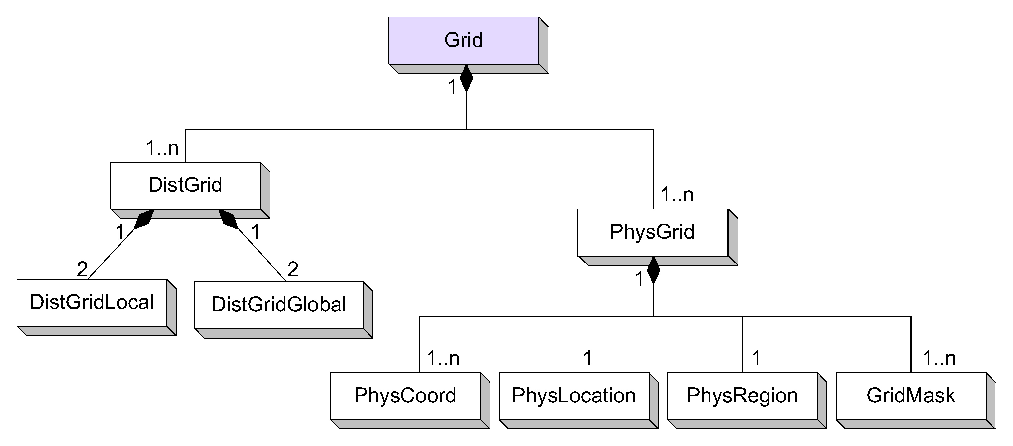
\includegraphics{Grid_obj.eps}   
\end{center}

Each Grid contains a Distributed Grid and a Physical Grid. The Physical Grid
maintains information about the global coordinates. In general this data is
described implicitly by specifying the grid type and the corresponding
parameters. However it is possible that the Physical Grid must be completely
enumerated, perhaps in the case of assimilated data or unstructured data. The
Distributed Grid defines an index space that corresponds to cells in 
the Physical
Grid and is decomposed among DEs in a DELayout.





% \section{Global Parameters and Definitions}
% #ifdef 1 
% \input{Grid_param}
% #elif defined(CONSTITUENT)
% \input{comppath/Grid_param}
% #endif

\section{Grid Design}

\subsection{Description}

% $Id: Grid_desc.tex,v 1.24 2007/03/31 05:51:08 cdeluca Exp $
%
% Earth System Modeling Framework
% Copyright 2002-2007, University Corporation for Atmospheric Research, 
% Massachusetts Institute of Technology, Geophysical Fluid Dynamics 
% Laboratory, University of Michigan, National Centers for Environmental 
% Prediction, Los Alamos National Laboratory, Argonne National Laboratory, 
% NASA Goddard Space Flight Center.
% Licensed under the University of Illinois-NCSA License.

% <Describe class function and relation to other classes.>

The ESMF Grid class represents all aspects of the computational domain and its
decomposition in a parallel-processing environment, and must provide access to
any necessary grid information to the rest of the ESMF.  The ESMF Grid class
is included in the Field class and the Gridded Component class
and provides information needed in data communication methods like halo and
redistribution.  It has methods to internally generate a variety of
simple grids or read in more complicated grids provided by a user 
(reading in grids is not yet implemented).  The ESMF Grid class supports
multi-component coupling by providing a common structure necessary for regridding.

ESMF Grids are currently assumed to be two-dimensional, logically-rectangular
horizontal grids, with an optional vertical grid whose coordinates are
independent of those of the horizontal grid.  Each Grid is assigned a
staggering in its create method call, which helps define the Grid according
to typical Arakawa nomenclature.  The staggering of the Grid sets the possible
relative locations ({\tt ESMF\_Rellocs}) for the Fields associated with that
Grid.  This interaction between Grid and data placement is explained in detail
in Section~\ref{sec:GridDataPlacement}.

ESMF differentiates between global data, which describes a complete set of data,
and DE-local data, which describes a distributed or decomposed chuck of data
located on a single DE.  The Grid class plays an integral role in this concept.
A Grid is first instantiated, via a create call, on all DEs in its domain, but
only in a global sense.  By that we mean it stores only information about the
global Grid, such as the number of grid cells and the coordinate extents, but
has not generated all the information that will end up distributed, such as the
cell coordinates.  The Grid is then decomposed onto a given DELayout via an
{\tt ESMF\_Distribute()} call.  At that point, the DE-local data types are
created and computed, so that on each DE there resides necessary global Grid
information as well as its own DE-local Grid data.  The DE-local data represented
by an {\tt ESMF\_Field} is defined by the decomposition of the underlying
{\tt ESMF\_Grid}.

\subsubsection{Grids and Data Placement}
\label{sec:GridDataPlacement}
An {\tt ESMF\_Grid} will support data placement only at specific cell relative
locations, defined by its staggering and following typical Arakawa nomenclature.
In ESMF, there are nine possible relative locations for data on a typical
horizontal Grid cell, though each staggering will use a subset of them.  These
locations, with their corresponding {\tt ESMF\_Rellocs}, are illustrated in
Figure~\ref{fig:GridDataLocations}.

\begin{center}
\begin{figure}
\scalebox{0.9}{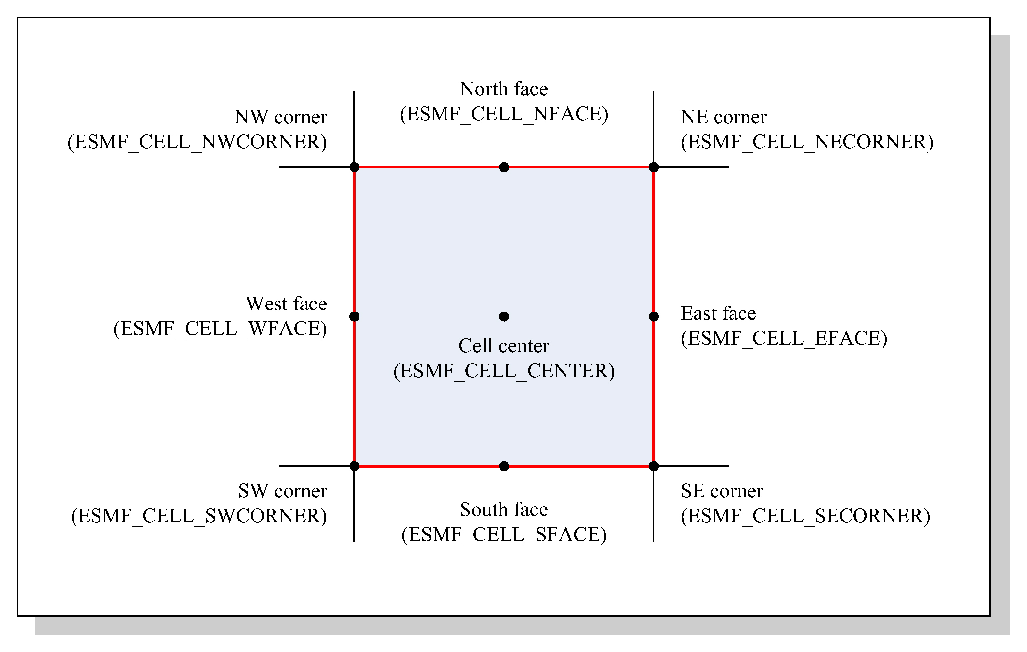
\includegraphics{GridDataLocations}}
\caption{Possible horizontal data locations for a representative computational
cell. }
\label{fig:GridDataLocations}
\end{figure}
\end{center}

{\tt ESMF\_Grids} are created with only those underlying structures, called
subGrids, to support data at the specific cell locations defined by its given
staggering.  For example, an Arakawa C grid has some computational fields
defined at the cell centers and other fields defined at specific cell face
centers.  An {\tt ESMF\_Grid} created with Arakawa C staggering will therefore
make subGrids at the cell centers and specified cell faces (please see
Section~\ref{sec:GridHorzStagger} for a complete list of implemented staggerings
and their corresponding Rellocs).  An example of the data locations for an
Arakawa C\_SE Grid is presented in Figure~\ref{fig:ArakawaC_SE}.

\begin{center}
\begin{figure}
\scalebox{0.9}{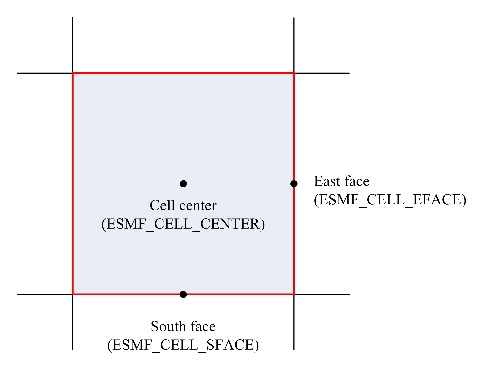
\includegraphics{ArakawaC_SE}}
\caption{Data locations for an Arakawa C\_SE Grid.}
\label{fig:ArakawaC_SE}
\end{figure}
\end{center}

A vertical grid is also represented as one or more subGrids, each corresponding
to a specific relative location along the defined vertical axis.  The possible
vertical relative locations are shown in Figure~\ref{fig:VertGridDataLocations}.

\begin{center}
\begin{figure}
\scalebox{0.9}{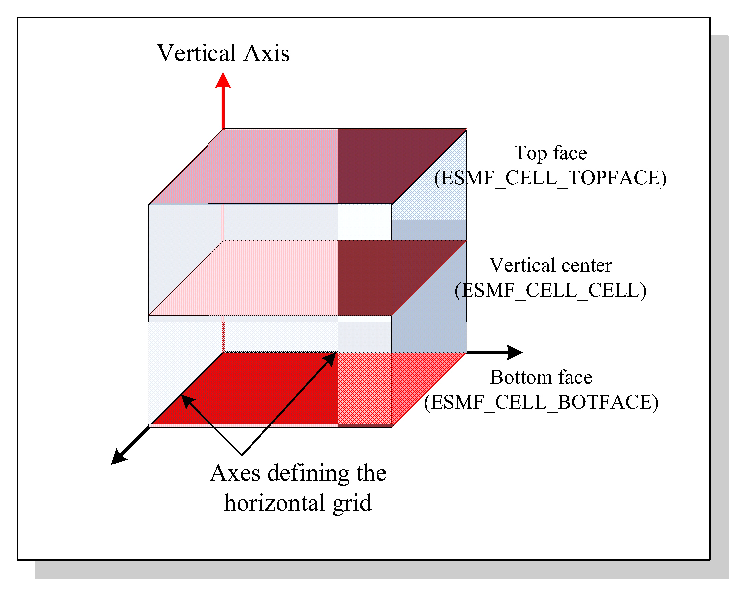
\includegraphics{VertGridDataLocations}}
\caption{Possible vertical data locations for a representative computational cell. }
\label{fig:VertGridDataLocations}
\end{figure}
\end{center}

Note that the locations in the figure are represented by horizontal planes.  The
vertical relative location only defines the vertical coordinate of any point, and
does not restrict the horizontal coordinates.  This means that the horizontal and
vertical Rellocs are independent of each other and can be combined in any way.
For a complete list of implemented vertical staggerings and their corresponding
Rellocs, please see Section~\ref{sec:GridVertStagger}.

The staggering of the Grid limits the relative locations of any ESMF data 
class corresponding to it.  When an {\tt ESMF\_Field} is created, it must be
assigned to one (or more, in the case of a horizontal Grid with a vertical
subGrid) of the appropriate subGrids present in the {\tt ESMF\_Grid} from
which it is being created.  Continuing the example above, an {\tt ESMF\_Field}
created from a Grid with Arakawa C staggering would have to be defined at either the cell center or one of the prescribed cell faces. 


\subsubsection{Grid Distribution}

The distribution (also referred to as decomposition) of the Grid on an
{\tt ESMF\_DELayout} determines the distribution as well for all related
ESMF data classes.  ESMF has currently implemented two different distribution
strategies: block and arbitrary.  In block distribution, logically rectangular
chunks of the global Grid are represented as local decomposition elements
(DEs), as shown in Figure~\ref{fig:GridBlockDistribute}.

\begin{center}
\begin{figure}
\scalebox{0.9}{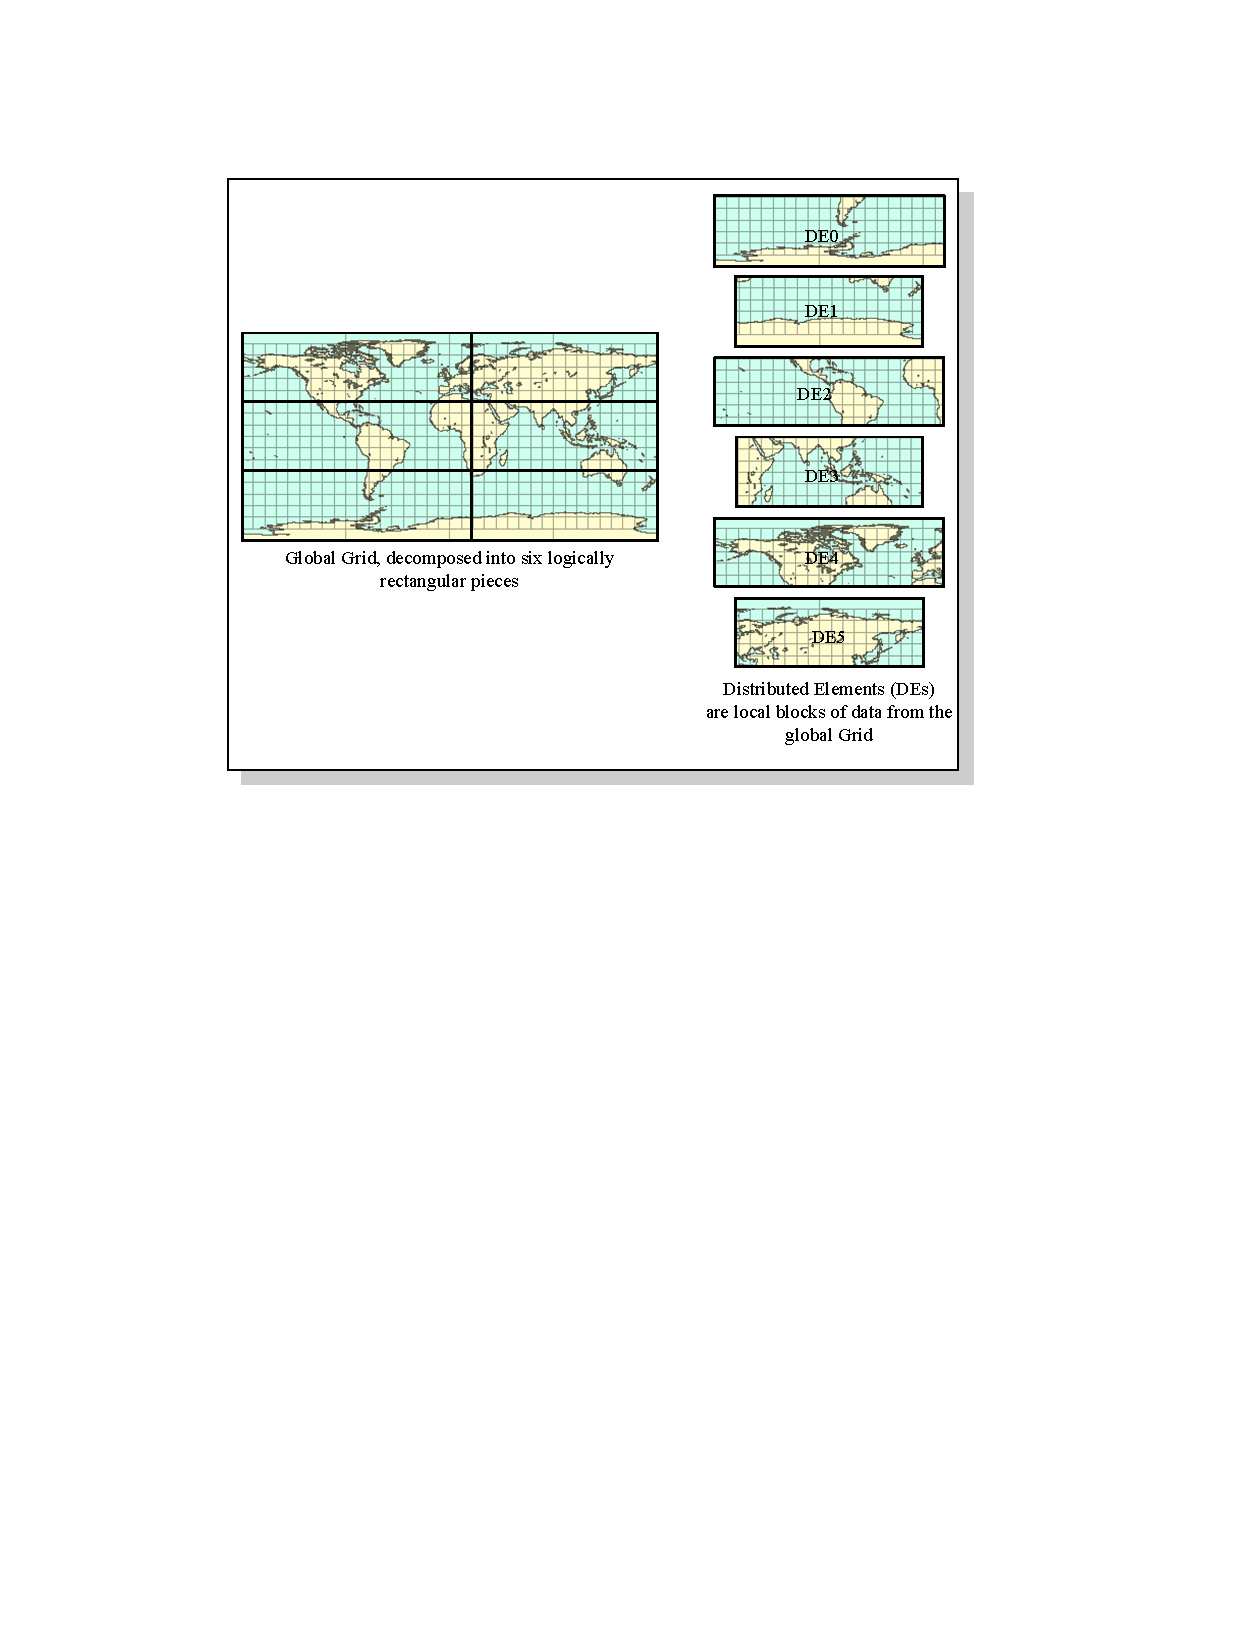
\includegraphics{GridBlockDistribution}}
\caption{Illustration of Block Distribution of a Grid. }
\label{fig:GridBlockDistribute}
\end{figure}
\end{center}

In this distribution method, some of the geometry and connectivity of the global
Grid are also true locally, in that most relative neighbor relationships are
maintained.  In arbitrary distribution, on the other hand, this is not
necessarily so, since the user specifies lists of individual points to
be grouped as DEs, as shown in Figure~\ref{fig:GridArbitraryDistribute}.

\begin{center}
\begin{figure}
\scalebox{0.9}{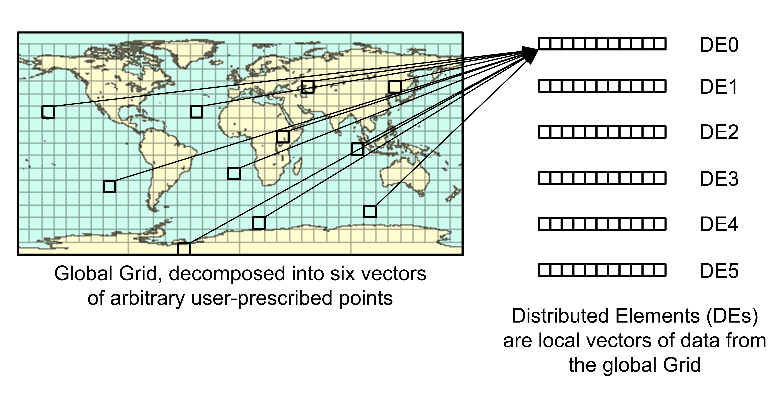
\includegraphics{GridArbitraryDistribution}}
\caption{Illustration of Arbitrary Distribution of a Grid. }
\label{fig:GridArbitraryDistribute}
\end{figure}
\end{center}

This method of distribution maintains local lists of cells without any sense
of their relationship to one another beyond their global index.  For that
reason, some higher level communication methods (like halo) would be 
inefficient for arbitrarily distributed Grids and their corresponding data
classes.  ESMF has implemented this distribution primarily to support 
components with column physics, which typically do not require much 
communication.  Currently for these objects ESMF only supports redistribution
between itself and a block distribution of the same global Grid to allow users
to move data from one representation to the other.



\subsection{Design}

% $Id$

%\subsection{Design}

% <Describe strategy for overall class design.>

Each Grid contains at least one Distributed Grid and one Physical Grid, both
of which are private classes.
The separation into two internal classes allows the code to differentiate
between functions which define the DE-local decomposition of data and
the DE-local representation of the grid.  The Grid class itself maintains
general information about the global Grid (e.g. the grid type, staggering,
and coordinate system).  The Grid class is relatively thin and
otherwise presents a unified interface for DistGrid and PhysGrid
functions.

The Grid class contains all information about the computational grid
for a Component, and must provide access to any necessary Grid information
to the rest of the ESMF.  A single Grid can have more than one related
DistGrid and PhysGrid set, called a subGrid.  Each subGrid corresponds to
a different representation of the Grid.  For example, a staggered Grid could
have separate subGrids representing cell centers and cell vertices.  A
vertical grid may also be represented as a subGrid.

Some methods which have a Grid interface are actually implemented
at the underlying DistGrid or PhysGrid level; they will be inherited
by the Grid class.  This allows the user API (Application Programming
Interface) to present functions at the level which is most consistent
to the application without restricting where inside the ESMF the actual
implementation is done.



\subsubsection{Class Definition}

% $Id: Grid_def.tex,v 1.2 2003/01/15 23:18:24 jwolfe Exp $

%\subsubsection{Class Definition}

See the beginning of the interface section which
follows for the definition of the Grid derived type
in Fortran 90, and the Field class in C++.





\subsubsection{Restrictions}

% $Id: Grid_rest.tex,v 1.3 2007/05/23 15:30:40 cdeluca Exp $

%\subsubsection{Restrictions and Future Work}

\begin{itemize}

\item {\bf 7D limit.}  Only grids up to 7D will be supported.

\item {\bf During the first development phase only single
tile grids are supported.}  In the near future, support
for mosaic grids will be added.  The initial implementation 
will be to create mosaics that contain tiles of the same
grid type, e.g. rectilinear.

\item {\bf Future adaptation.}  Currently Grids
are created and then remain unchanged. In the future, it would
be useful to provide support for the various forms of grid
adaptation. This would allow the grids to dynamically change
their resolution to more closely match what is needed at a particular
time and postion during a computation for front tracking or adaptive meshes.

\item {\bf Future Grid masks.}  Grid masks will be implemented.

\item {\bf Future Exchange Grids.}  The functionality for creating an 
exchange grid between two ordinary grids will be implemented
to assist with the remapping of data during a regrid operation. 

\item {\bf Future unstructured Grid.}  Currently only grids which can be constructed from a set of logically rectangular tiles are supported. In the future more general unstructured grids will be implemented.

\item {\bf Future Grid IO.} In the future it would be useful to have a grid method which can read in a grid specification and distribution from a file and construct the grid. There may need to be a set of these methods corresponding to different group's file formats.

\item {\bf Future Grid generation.} This class for now only contains
the basic functionality for operating on the grid. In the future
methods will be added to enable the automatic generation of various types of
grids. 


\end{itemize}




\section{Grid F90 Interface}

\subsection{Use and Examples}

% $Id: Grid_fex.tex,v 1.1 2002/12/03 23:27:18 jwolfe Exp $

%\subsection{F90 Use and Examples}

See the following code fragment for an example of
how to use Grid.  Also see
the Programming Model section of this document.






\subsection{Parameters and Definitions}

% $Id: Grid_fparam.tex,v 1.1 2002/12/03 23:27:45 jwolfe Exp $

%\subsection{Parameters}

\begin{description}

\item [Grid] A Grid derived type is the following:
\begin{verbatim}
type ESMF_Grid
sequence
end type
\end{verbatim}


\end{description}






%\subsection{Class API}

%                **** IMPORTANT NOTICE *****
% This LaTeX file has been automatically produced by ProTeX v. 1.1
% Any changes made to this file will likely be lost next time
% this file is regenerated from its source. Send questions 
% to Arlindo da Silva, dasilva@gsfc.nasa.gov
 
\parskip        0pt
\parindent      0pt
\baselineskip  11pt
 
%--------------------- SHORT-HAND MACROS ----------------------
\def\bv{\begin{verbatim}}
\def\ev{\end{verbatim}}
\def\be{\begin{equation}}
\def\ee{\end{equation}}
\def\bea{\begin{eqnarray}}
\def\eea{\end{eqnarray}}
\def\bi{\begin{itemize}}
\def\ei{\end{itemize}}
\def\bn{\begin{enumerate}}
\def\en{\end{enumerate}}
\def\bd{\begin{description}}
\def\ed{\end{description}}
\def\({\left (}
\def\){\right )}
\def\[{\left [}
\def\]{\right ]}
\def\<{\left  \langle}
\def\>{\right \rangle}
\def\cI{{\cal I}}
\def\diag{\mathop{\rm diag}}
\def\tr{\mathop{\rm tr}}
%-------------------------------------------------------------

\markboth{Left}{Source File: ESMF\_Grid.F90,  Date: Thu Jan 16 12:11:35 MST 2003
}

 
%/////////////////////////////////////////////////////////////
\subsection{Fortran:  Module Interface ESMF\_GridMod - Grid class (Source File: ESMF\_Grid.F90)}


  
  
   The code in this file implements the {\tt Grid} class.  This class
   provides a unified interface for both {\tt PhysGrid} and {\tt DistGrid}
   information for model grids.  Functions for defining and computing {\tt Grid}
   information are available through this class.
  
  ------------------------------------------------------------------------------
\bigskip{\em USES:}
\begin{verbatim}       use ESMF_ArrayMod       ! ESMF array class
       use ESMF_BaseMod        ! ESMF base class
       use ESMF_DistGridMod    ! ESMF distributed grid class
       use ESMF_IOMod          ! ESMF I/O class
       use ESMF_LayoutMod      ! ESMF layout class
       use ESMF_PhysGridMod    ! ESMF physical grid class
       implicit none
 
  ------------------------------------------------------------------------------\end{verbatim}{\sf PRIVATE TYPES:}
\begin{verbatim}       private
  ------------------------------------------------------------------------------
       ! ESMF_GridConfig
       ! Description of ESMF_GridConfig
 
       type ESMF_GridConfig
       sequence
       private
         integer :: dummy
         < insert other class members here >
       end type
 
  ------------------------------------------------------------------------------
       !  ESMF_GridType
       ! Definition for the Grid class.  A Grid
       ! is passed back to the user at Grid creation.
 
       type ESMF_GridType
       sequence
       private
 
         type (ESMF_Base) :: base            ! base class object
         type (ESMF_Status) :: gridstatus    ! uninitialized, init ok, etc
         integer :: horz_gridtype            ! enum for type of horizontal grid
         integer :: vert_gridtype            ! enum for type of vertical grid
         integer :: horz_stagger             ! enum for horizontal grid staggering
         integer :: vert_stagger             ! enum for vertical grid staggering
         integer :: horz_coord_system        ! enum for horizontal physical
                                             ! coordinate system
         integer :: vert_coord_system        ! enum for vertical physical
                                             ! coordinate system
         integer :: coord_order              ! enum for mapping of xyz 
                                             ! to ijk
         integer :: coord_index              ! enum for global or local indexing
         integer :: num_physgrids            ! number of grid descriptors
                                             ! necessary to support
                                             ! staggering, vertical
                                             ! grids, background grids
         type (ESMF_PhysGridType), dimension(:), pointer :: &
            physgrids         ! grid info for all grid descriptions necessary
                              ! to define horizontal, staggered and vertical grids
         type (ESMF_DistGrid) :: distgrid    ! decomposition and other
                                             ! logical space info for grid
         type (???) :: search_structure
 
       end type
 
  ------------------------------------------------------------------------------
       !  ESMF_Grid
       ! The Grid data structure that is passed between languages.
 
       type ESMF_Grid
       sequence
       private
         type (ESMF_GridType), pointer :: ptr     ! pointer to a grid type
       end type
 
  ------------------------------------------------------------------------------\end{verbatim}{\sf PUBLIC TYPES:}
\begin{verbatim} 
       public ESMF_GridConfig
       public ESMF_Grid
       public ESMF_GridType
 
  ------------------------------------------------------------------------------\end{verbatim}{\sf PUBLIC MEMBER FUNCTIONS:}
\begin{verbatim} 
     public ESMF_GridCreate
     public ESMF_GridDestroy
     public ESMF_GridAddPhysGrid
     public ESMF_GridGetConfig
     public ESMF_GridSetConfig
     !public ESMF_GridGetCoord
     public ESMF_GridSetCoord
     public ESMF_GridGetDE    ! temporary to access DistGrid from above
     !public ESMF_GridGetInfo
     public ESMF_GridSetInfo
     !public ESMF_GridGetLMask
     public ESMF_GridSetLMask
     !public ESMF_GridGetMMask
     public ESMF_GridSetMMask
     !public ESMF_GridGetMetric
     public ESMF_GridSetMetric
     !public ESMF_GridGetRegionID
     public ESMF_GridSetRegionID
     public ESMF_GridValidate
     public ESMF_GridPrint
 
  ------------------------------------------------------------------------------\end{verbatim}{\sf PUBLIC DATA MEMBERS:}
\begin{verbatim} 
    integer, parameter, public ::            &! recognized grid types
       ESMF_GridType_Unknown           =  0, &! unknown or undefined grid
       ESMF_GridType_LatLon            =  1, &! equally-spaced lat/lon grid
       ESMF_GridType_Mercator          =  2, &! Mercator lat/lon grid
       ESMF_GridType_Dipole            =  3, &! Displaced-pole dipole grid
       ESMF_GridType_Tripole           =  4, &! Tripolar grids
       ESMF_GridType_XY                =  5, &! Cartesian equally-space x-y grid
       ESMF_GridType_DataStream        =  6, &! Data stream
       ESMF_GridType_PhysFourier       =  7, &! Mixed Fourier Space/Phys Space grid
       ESMF_GridType_LatLonGauss       =  8, &! lat/lon grid with Gaussian latitudes
       ESMF_GridType_SphericalSpectral =  9, &! spectral space for spherical harmonics
       ESMF_GridType_Geodesic          = 10, &! spherical geodesic grid
       ESMF_GridType_CubedSphere       = 11   ! cubed sphere grid
 
    integer, parameter, public ::            &! recognized staggering types
       ESMF_GridStagger_Unknown        =  0, &! unknown or undefined staggering
       ESMF_GridStagger_A              =  1, &! Arakawa A (centered velocity)
       ESMF_GridStagger_B              =  2, &! Arakawa B (velocities at grid corner)
       ESMF_GridStagger_C              =  3, &! Arakawa C (velocities at cell faces)
       ESMF_GridStagger_Z              =  4, &! C grid equiv for geodesic grid
       ESMF_GridStagger_VertCenter     =  5, &! vert velocity at vertical midpoints
       ESMF_GridStagger_VertFace       =  6   ! vert velocity/Pgrad at top(bottom)face
 
    integer, parameter, public ::            &! recognized coordinate systems
       ESMF_CoordSystem_Unknown        =  0, &! unknown or undefined coord system
       ESMF_CoordSystem_Spherical      =  1, &! spherical coordinates (lat/lon)
       ESMF_CoordSystem_Cartesian      =  2, &! Cartesian coordinates (x,y)
       ESMF_CoordSystem_Cylindrical    =  3, &! cylindrical coordinates
       ESMF_CoordSystem_LatFourier     =  4, &! mixed latitude/spectral space
       ESMF_CoordSystem_Spectral       =  5, &! wavenumber space
       ESMF_CoordSystem_Depth          =  6, &! vertical z coord. depth (0 at surface)
       ESMF_CoordSystem_Height         =  7, &! vertical z coord. height (0 at bottom)
       ESMF_CoordSystem_Pressure       =  8, &! vertical pressure coordinate
       ESMF_CoordSystem_Sigma          =  9, &! vertical sigma coordinate
       ESMF_CoordSystem_Theta          = 10, &! vertical theta coordinate
       ESMF_CoordSystem_Eta            = 11, &! vertical eta coordinate
       ESMF_CoordSystem_Isopycnal      = 12, &! vertical density coordinate
       ESMF_CoordSystem_Hybrid         = 13, &! hybrid vertical coordinates
       ESMF_CoordSystem_Lagrangian     = 14   ! Lagrangian coordinates
       ! I'm sure there are more - I'm not sure
       ! what the atmospheric ESMF models are using for vertical coords
 
    integer, parameter, public ::            &! recognized coordinate orderings
       ESMF_CoordOrder_Unknown         =  0, &! unknown or undefined coord ordering
       ESMF_CoordOrder_XYZ             =  1, &! IJK maps to XYZ
       ESMF_CoordOrder_XZY             =  2, &! IJK maps to XZY
       ESMF_CoordOrder_YXZ             =  3, &! IJK maps to YXZ
       ESMF_CoordOrder_YZX             =  4, &! IJK maps to YZX
       ESMF_CoordOrder_ZXY             =  5, &! IJK maps to ZXY
       ESMF_CoordOrder_ZYX             =  6   ! IJK maps to ZYX
 
    integer, parameter, public ::            &! recognized coordinate indexings
       ESMF_CoordIndex_Unknown         =  0, &! unknown or undefined coord indexing
       ESMF_CoordIndex_Local           =  1, &! uses local indexing
       ESMF_CoordIndex_Global          =  2   ! uses global indexing
 \end{verbatim}
 
%/////////////////////////////////////////////////////////////
 
\mbox{}\hrulefill\ 
 

\bigskip{\sf INTERFACE:}
\begin{verbatim}       interface ESMF_GridCreate
 \end{verbatim}{\sf PRIVATE MEMBER FUNCTIONS:}
\begin{verbatim}          module procedure ESMF_GridCreateEmpty
          module procedure ESMF_GridCreateInternal
          module procedure ESMF_GridCreateRead
          module procedure ESMF_GridCreateCopy
          module procedure ESMF_GridCreateCutout
          module procedure ESMF_GridCreateChangeResolution
          module procedure ESMF_GridCreateExchange
 \end{verbatim}
{\sf DESCRIPTION:\\ }


       This interface provides a single entry point for {\tt Grid} create
       methods.
   
%/////////////////////////////////////////////////////////////
 
\mbox{}\hrulefill\ 
 

\bigskip{\sf INTERFACE:}
\begin{verbatim}       interface ESMF_GridConstruct
 \end{verbatim}{\sf PRIVATE MEMBER FUNCTIONS:}
\begin{verbatim}          module procedure ESMF_GridConstructNew
          module procedure ESMF_GridConstructInternal
 \end{verbatim}
{\sf DESCRIPTION:\\ }


       This interface provides a single entry point for methods that construct a
       complete {\tt Grid}.
   
%/////////////////////////////////////////////////////////////
 
\mbox{}\hrulefill\ 
 

\bigskip{\sf INTERFACE:}
\begin{verbatim}       interface ESMF_GridSetCoord
 \end{verbatim}{\sf PRIVATE MEMBER FUNCTIONS:}
\begin{verbatim}          module procedure ESMF_GridSetCoordFromArray
          module procedure ESMF_GridSetCoordFromBuffer
          module procedure ESMF_GridSetCoordCompute
          module procedure ESMF_GridSetCoordCopy
 \end{verbatim}
{\sf DESCRIPTION:\\ }


       This interface provides a single entry point for methods that set
       coordinates as part of a {\tt Grid}.
   
%/////////////////////////////////////////////////////////////
 
\mbox{}\hrulefill\ 
 

\bigskip{\sf INTERFACE:}
\begin{verbatim}       interface ESMF_GridSetLMask
 \end{verbatim}{\sf PRIVATE MEMBER FUNCTIONS:}
\begin{verbatim}          module procedure ESMF_GridSetLMaskFromArray
          module procedure ESMF_GridSetLMaskFromBuffer
          module procedure ESMF_GridSetLMaskFromMMask
          module procedure ESMF_GridSetLMaskCopy
 \end{verbatim}
{\sf DESCRIPTION:\\ }


       This interface provides a single entry point for methods that set
       logical masks as part of a {\tt Grid}.
   
%/////////////////////////////////////////////////////////////
 
\mbox{}\hrulefill\ 
 

\bigskip{\sf INTERFACE:}
\begin{verbatim}       interface ESMF_GridSetMMask
 \end{verbatim}{\sf PRIVATE MEMBER FUNCTIONS:}
\begin{verbatim}          module procedure ESMF_GridSetMMaskFromArray
          module procedure ESMF_GridSetMMaskFromBuffer
          module procedure ESMF_GridSetMMaskFromLMask
          module procedure ESMF_GridSetMMaskCopy
 \end{verbatim}
{\sf DESCRIPTION:\\ }


       This interface provides a single entry point for methods that set
       multiplicative masks as part of a {\tt Grid}.
   
%/////////////////////////////////////////////////////////////
 
\mbox{}\hrulefill\ 
 

\bigskip{\sf INTERFACE:}
\begin{verbatim}       interface ESMF_GridSetMetric
 \end{verbatim}{\sf PRIVATE MEMBER FUNCTIONS:}
\begin{verbatim}          module procedure ESMF_GridSetMetricFromArray
          module procedure ESMF_GridSetMetricFromBuffer
          module procedure ESMF_GridSetMetricCompute
          module procedure ESMF_GridSetMetricCopy
 \end{verbatim}
{\sf DESCRIPTION:\\ }


       This interface provides a single entry point for methods that set
       metrics as part of a {\tt Grid}.
   
%/////////////////////////////////////////////////////////////
 
\mbox{}\hrulefill\ 
 

\bigskip{\sf INTERFACE:}
\begin{verbatim}       interface ESMF_GridSetRegionID
 \end{verbatim}{\sf PRIVATE MEMBER FUNCTIONS:}
\begin{verbatim}          module procedure ESMF_GridSetRegionIDFromArray
          module procedure ESMF_GridSetRegionIDFromBuffer
          module procedure ESMF_GridSetRegionIDCopy
 \end{verbatim}
{\sf DESCRIPTION:\\ }


       This interface provides a single entry point for methods that set
       region id's as part of a {\tt Grid}.
   
%/////////////////////////////////////////////////////////////
 
\mbox{}\hrulefill\ 
 
\subsubsection{ESMF\_GridCreateEmpty - Create a new Grid with no data}


 
\bigskip{\sf INTERFACE:}
\begin{verbatim}       function ESMF_GridCreateEmpty(name, rc)\end{verbatim}{\em RETURN VALUE:}
\begin{verbatim}       type(ESMF_Grid) :: ESMF_GridCreateEmpty\end{verbatim}{\em ARGUMENTS:}
\begin{verbatim}       character (len=*), intent(in), optional :: name
       integer, intent(out), optional :: rc\end{verbatim}
{\sf DESCRIPTION:\\ }


       Allocates memory for a new {\tt Grid} object and constructs its
       internals.  Return a pointer to the new {\tt Grid}.
  
       The arguments are:
       \begin{description}
       \item[[name]]
            {\tt Grid} name.
       \item[[rc]]
            Return code; equals {\tt ESMF\_SUCCESS} if there are no errors.
     \end{description}
  
\bigskip{\sf REQUIREMENTS:}
\begin{verbatim} \end{verbatim}
 
%/////////////////////////////////////////////////////////////
 
\mbox{}\hrulefill\ 
 
\subsubsection{ESMF\_GridCreateInternal - Create a new Grid internally}


\bigskip{\sf INTERFACE:}
\begin{verbatim}       function ESMF_GridCreateInternal(i_max, j_max, &
                                        nDE_i, nDE_j, layout, &
                                        horz_gridtype, vert_gridtype, &
                                        horz_stagger, vert_stagger, &
                                        horz_coord_system, vert_coord_system, &
                                        x_min, x_max, y_min, y_max, name, rc)\end{verbatim}{\em RETURN VALUE:}
\begin{verbatim}       type(ESMF_Grid) :: ESMF_GridCreateInternal\end{verbatim}{\em ARGUMENTS:}
\begin{verbatim}       integer, intent(in) :: i_max
       integer, intent(in) :: j_max
       integer, intent(in), optional :: nDE_i
       integer, intent(in), optional :: nDE_j
       type (ESMF_Layout), intent(in), optional :: layout
       integer, intent(in), optional :: horz_gridtype
       integer, intent(in), optional :: vert_gridtype
       integer, intent(in), optional :: horz_stagger
       integer, intent(in), optional :: vert_stagger
       integer, intent(in), optional :: horz_coord_system
       integer, intent(in), optional :: vert_coord_system
       real, intent(in), optional :: x_min
       real, intent(in), optional :: x_max
       real, intent(in), optional :: y_min
       real, intent(in), optional :: y_max
       character (len=*), intent(in), optional :: name
       integer, intent(out), optional :: rc\end{verbatim}
{\sf DESCRIPTION:\\ }


       Allocates memory for a new {\tt Grid} object, constructs its
       internals, and internally generates the Grid.  Return a pointer to
       the new {\tt Grid}.
  
       The arguments are:
       \begin{description}
       \item[[i\_max]]
            Number of grid increments in the i-direction.
       \item[[j\_max]]
            Number of grid increments in the j-direction.
       \item[[nDE\_i]]
            Number of DE's in 1st dir.
       \item[[nDE\_j]]
            Number of DE's in 2nd dir.
       \item[[layout]]
            Layout of DE's.
       \item[[horz\_gridtype]]
            Integer specifier to denote horizontal gridtype.
       \item[[vert\_gridtype]]
            Integer specifier to denote vertical gridtype.
       \item[[horz\_stagger]]
            Integer specifier to denote horizontal grid stagger.
       \item[[vert\_stagger]]
            Integer specifier to denote vertical grid stagger.
       \item[[horz\_coord\_system]]
            Integer specifier to denote horizontal coordinate system.
       \item[[vert\_coord\_system]]
            Integer specifier to denote vertical coordinate system.
       \item[[x\_min]]
            Minimum physical coordinate in the x-direction.
       \item[[x\_max]]
            Maximum physical coordinate in the x-direction.
       \item[[y\_min]]
            Minimum physical coordinate in the y-direction.
       \item[[y\_max]]
            Maximum physical coordinate in the y-direction.
       \item[[name]]
            {\tt Grid} name.
       \item[[rc]]
            Return code; equals {\tt ESMF\_SUCCESS} if there are no errors.
     \end{description}
  
\bigskip{\sf REQUIREMENTS:}
\begin{verbatim} \end{verbatim}
 
%/////////////////////////////////////////////////////////////
 
\mbox{}\hrulefill\ 
 
\subsubsection{ESMF\_GridCreateRead - Create a new Grid read in from a file}


\bigskip{\sf INTERFACE:}
\begin{verbatim}       function ESMF_GridCreateRead(iospec, name, rc)\end{verbatim}{\em RETURN VALUE:}
\begin{verbatim}       type(ESMF_Grid) :: ESMF_GridCreateRead\end{verbatim}{\em ARGUMENTS:}
\begin{verbatim}       type(ESMF_IOSpec), intent(in) :: iospec   ! file specs
       character (len=*), intent(in), optional :: name
       integer, intent(out), optional :: rc\end{verbatim}
{\sf DESCRIPTION:\\ }


       Allocates memory for a new {\tt Grid} object, constructs its
       internals, and reads a {\tt Grid} in from a file.  Return a pointer to
       the new {\tt Grid}.
  
       The arguments are:
       \begin{description}
       \item[[iospec]]
            File I/O specification.
       \item[[name]]
            {\tt Grid} name.
       \item[[rc]]
            Return code; equals {\tt ESMF\_SUCCESS} if there are no errors.
     \end{description}
  
\bigskip{\sf REQUIREMENTS:}
\begin{verbatim} \end{verbatim}
 
%/////////////////////////////////////////////////////////////
 
\mbox{}\hrulefill\ 
 
\subsubsection{ESMF\_GridCreateCopy - Create a new Grid by copying another Grid}


\bigskip{\sf INTERFACE:}
\begin{verbatim}       function ESMF_GridCreateCopy(grid_in, name, rc)\end{verbatim}{\em RETURN VALUE:}
\begin{verbatim}       type(ESMF_Grid) :: ESMF_GridCreateCopy\end{verbatim}{\em ARGUMENTS:}
\begin{verbatim}       type(ESMF_Grid), intent(in) :: grid_in
       character (len=*), intent(in), optional :: name
       integer, intent(out), optional :: rc\end{verbatim}
{\sf DESCRIPTION:\\ }


       Allocates memory for a new {\tt Grid} object, constructs its
       internals, and copies attributes from another {\tt Grid}.  Return a
       pointer to the new {\tt Grid}.
  
       The arguments are:
       \begin{description}
       \item[[grid\_in]]
            {\tt Grid} to be copied.
       \item[[name]]
            {\tt Grid} name.
       \item[[rc]]
            Return code; equals {\tt ESMF\_SUCCESS} if there are no errors.
     \end{description}
  
\bigskip{\sf REQUIREMENTS:}
\begin{verbatim} \end{verbatim}
 
%/////////////////////////////////////////////////////////////
 
\mbox{}\hrulefill\ 
 
\subsubsection{ESMF\_GridCreateCutout - Create a new Grid as a subset of an existing Grid}


\bigskip{\sf INTERFACE:}
\begin{verbatim}       function ESMF_GridCreateCutout(grid_in, i_min, i_max, j_min, j_max, &
                                      name, rc)\end{verbatim}{\em RETURN VALUE:}
\begin{verbatim}       type(ESMF_Grid) :: ESMF_GridCreateCutout\end{verbatim}{\em ARGUMENTS:}
\begin{verbatim}       type(ESMF_Grid), intent(in) :: grid_in
       integer, intent(in) :: i_min
       integer, intent(in) :: i_max
       integer, intent(in) :: j_min
       integer, intent(in) :: j_max
       character (len=*), intent(in), optional :: name
       integer, intent(out), optional :: rc\end{verbatim}
{\sf DESCRIPTION:\\ }


       Allocates memory for a new {\tt Grid} object, constructs its
       internals, and copies a region from an existing {\tt Grid}.
       Return a pointer to the new {\tt Grid}.
  
       The arguments are:
       \begin{description}
       \item[[grid\_in]]
            {\tt Grid} to be partially copied.
       \item[[i\_min]]
            Minimum global i-index for the region of the grid to be cutout.
       \item[[i\_max]]
            Maximum global i-index for the region of the grid to be cutout.
       \item[[j\_min]]
            Minimum global j-index for the region of the grid to be cutout.
       \item[[j\_max]]
            Maximum global j-index for the region of the grid to be cutout.
       \item[[name]]
            {\tt Grid} name.
       \item[[rc]]
            Return code; equals {\tt ESMF\_SUCCESS} if there are no errors.
     \end{description}
  
\bigskip{\sf REQUIREMENTS:}
\begin{verbatim} \end{verbatim}
 
%/////////////////////////////////////////////////////////////
 
\mbox{}\hrulefill\ 
 
\subsubsection{ESMF\_GridCreateChangeResolution - Create a new Grid by coarsening or refining an existing Grid}


\bigskip{\sf INTERFACE:}
\begin{verbatim}       function ESMF_GridCreateChangeResolution(grid_in, i_resolution, &
                                                j_resolution, name, rc)\end{verbatim}{\em RETURN VALUE:}
\begin{verbatim}       type(ESMF_Grid) :: ESMF_GridCreateChangeResolution\end{verbatim}{\em ARGUMENTS:}
\begin{verbatim}       type(ESMF_Grid), intent(in) :: grid_in
       integer, intent(in) :: i_resolution
       integer, intent(in) :: j_resolution
       character (len=*), intent(in), optional :: name
       integer, intent(out), optional :: rc\end{verbatim}
{\sf DESCRIPTION:\\ }


       Allocates memory for a new {\tt Grid} object, constructs its
       internals, and creates a {\tt Grid} by either coarsening or refining an
       existing {\tt Grid}.  Return a pointer to the new {\tt Grid}.
  
       The arguments are:
       \begin{description}
       \item[[grid\_in]]
            Source {\tt Grid} to be coarsened or refined.
       \item[[i\_resolution]]
            Integer resolution factor in the i-direction.
       \item[[j\_resolution]]
            Integer resolution factor in the j-direction.
            Note:  The above arguments assume refinement by factor if positive
            and coarsening by absolute value of the factor if negative.  For
            example, i\_resolution=4 indicates the new {\tt Grid} will be four
            times as resolved in the i-direction as the source {\tt Grid},
            whereas j\_resolution=-3 means the new {\tt Grid} will sample every
            third point in the j-direction.
       \item[[name]]
            {\tt Grid} name.
       \item[[rc]]
            Return code; equals {\tt ESMF\_SUCCESS} if there are no errors.
     \end{description}
  
\bigskip{\sf REQUIREMENTS:}
\begin{verbatim} \end{verbatim}
 
%/////////////////////////////////////////////////////////////
 
\mbox{}\hrulefill\ 
 
\subsubsection{ESMF\_GridCreateExchange - Create a new Grid from the intersection of two existing grids}


\bigskip{\sf INTERFACE:}
\begin{verbatim}       function ESMF_GridCreateExchange(grid_in1, grid_in2, name, rc)\end{verbatim}{\em RETURN VALUE:}
\begin{verbatim}       type(ESMF_Grid) :: ESMF_GridCreateExchange\end{verbatim}{\em ARGUMENTS:}
\begin{verbatim}       type(ESMF_Grid), intent(in) :: grid_in1
       type(ESMF_Grid), intent(in) :: grid_in2
       character (len=*), intent(in), optional :: name
       integer, intent(out), optional :: rc\end{verbatim}
{\sf DESCRIPTION:\\ }


       Allocates memory for a new {\tt Grid} object, constructs its
       internals, and creates a new {\tt Grid} from the intersection of two
       existing {\tt Grids}.  Return a pointer to the new {\tt Grid}.
  
       The arguments are:
       \begin{description}
       \item[[grid\_in1]]
            First source {\tt Grid}.
       \item[[grid\_in2]]
            Second source {\tt Grid}.
       \item[[name]]
            New {\tt Grid} name.
       \item[[rc]]
            Return code; equals {\tt ESMF\_SUCCESS} if there are no errors.
     \end{description}
  
\bigskip{\sf REQUIREMENTS:}
\begin{verbatim} \end{verbatim}
 
%/////////////////////////////////////////////////////////////
 
\mbox{}\hrulefill\ 
 
\subsubsection{ESMF\_GridDestroy - Free all resources associated with a Grid }


\bigskip{\sf INTERFACE:}
\begin{verbatim}       subroutine ESMF_GridDestroy(grid, rc)\end{verbatim}{\em ARGUMENTS:}
\begin{verbatim}       type(ESMF_Grid), intent(in) :: grid
       integer, intent(out), optional :: rc\end{verbatim}
{\sf DESCRIPTION:\\ }


       Destroys a {\tt Grid} object previously allocated
       via an {\tt ESMF\_GridCreate routine}.
  
       The arguments are:
       \begin{description}
       \item[grid]
            The class to be destroyed.
       \item[[rc]]
            Return code; equals {\tt ESMF\_SUCCESS} if there are no errors.
       \end{description}
   
%/////////////////////////////////////////////////////////////
 
\mbox{}\hrulefill\ 
 
\subsubsection{ESMF\_GridConstructInternal - Construct the internals of an allocated Grid}


 
\bigskip{\sf INTERFACE:}
\begin{verbatim}       subroutine ESMF_GridConstructInternal(grid, i_max, j_max, &
                                             nDE_i, nDE_j, layout, &
                                             horz_gridtype, vert_gridtype, &
                                             horz_stagger, vert_stagger, &
                                             horz_coord_system, vert_coord_system, &
                                             x_min, x_max, y_min, y_max, name, rc)\end{verbatim}{\em ARGUMENTS:}
\begin{verbatim}       type(ESMF_GridType) :: grid
       integer, intent(in) :: i_max
       integer, intent(in) :: j_max
       integer, intent(in), optional :: nDE_i
       integer, intent(in), optional :: nDE_j
       type (ESMF_Layout), intent(in), optional :: layout
       integer, intent(in), optional :: horz_gridtype
       integer, intent(in), optional :: vert_gridtype
       integer, intent(in), optional :: horz_stagger
       integer, intent(in), optional :: vert_stagger
       integer, intent(in), optional :: horz_coord_system
       integer, intent(in), optional :: vert_coord_system
       real, intent(in), optional :: x_min
       real, intent(in), optional :: x_max
       real, intent(in), optional :: y_min
       real, intent(in), optional :: y_max
       character (len = *), intent(in), optional :: name
       integer, intent(out), optional :: rc\end{verbatim}
{\sf DESCRIPTION:\\ }


       ESMF routine which fills in the contents of an already
       allocated {\tt Grid} object.  May perform additional allocations
       as needed.  Must call the corresponding ESMF\_GridDestruct
       routine to free the additional memory.  Intended for internal
       ESMF use only; end-users use {\tt ESMF\_GridCreate}, which calls
       {\tt ESMF\_GridConstruct}.
  
       The arguments are:
       \begin{description}
       \item[grid]
            Pointer to a {\tt Grid}
       \item[[i\_max]]
            Number of grid increments in the i-direction.
       \item[[j\_max]]
            Number of grid increments in the j-direction.
       \item[[nDE\_i]]
            Number of DE's in 1st dir.
       \item[[nDE\_j]]
            Number of DE's in 2nd dir.
       \item[[layout]]
           Layout of DE's.
       \item[[horz\_gridtype]]
            Integer specifier to denote horizontal gridtype.
       \item[[vert\_gridtype]]
            Integer specifier to denote vertical gridtype.
       \item[[horz\_stagger]]
            Integer specifier to denote horizontal grid stagger.
       \item[[vert\_stagger]]
            Integer specifier to denote vertical grid stagger.
       \item[[horz\_coord\_system]]
            Integer specifier to denote horizontal coordinate system.
       \item[[vert\_coord\_system]]
            Integer specifier to denote vertical coordinate system.
       \item[[x\_min]]
            Minimum physical coordinate in the x-direction.
       \item[[x\_max]]
            Maximum physical coordinate in the x-direction.
       \item[[y\_min]]
            Minimum physical coordinate in the y-direction.
       \item[[y\_max]]
            Maximum physical coordinate in the y-direction.
       \item[[rc]]
            Return code; equals {\tt ESMF\_SUCCESS} if there are no errors.
       \end{description}
  
\bigskip{\sf REQUIREMENTS:}
\begin{verbatim} \end{verbatim}
 
%/////////////////////////////////////////////////////////////
 
\mbox{}\hrulefill\ 
 
\subsubsection{ESMF\_GridConstructNew - Construct the internals of an allocated Grid}


\bigskip{\sf INTERFACE:}
\begin{verbatim}       subroutine ESMF_GridConstructNew(grid, name, rc)\end{verbatim}{\em ARGUMENTS:}
\begin{verbatim}       type(ESMF_GridType) :: grid
       character (len = *), intent(in), optional :: name
       integer, intent(out), optional :: rc\end{verbatim}
{\sf DESCRIPTION:\\ }


       ESMF routine which fills in the contents of an already
       allocated {\tt Grid} object.  May perform additional allocations
       as needed.  Must call the corresponding ESMF\_GridDestruct
       routine to free the additional memory.  Intended for internal
       ESMF use only; end-users use {\tt ESMF\_GridCreate}, which calls
       {\tt ESMF\_GridConstruct}.
  
       The arguments are:
       \begin{description}
       \item[grid]
            Pointer to a {\tt Grid}
       \item[[name]]
            {\tt Grid} name.
       \item[[rc]]
            Return code; equals {\tt ESMF\_SUCCESS} if there are no errors.
       \end{description}
  
\bigskip{\sf REQUIREMENTS:}
\begin{verbatim} \end{verbatim}
 
%/////////////////////////////////////////////////////////////
 
\mbox{}\hrulefill\ 
 
\subsubsection{ESMF\_GridDestruct - Free any Grid memory allocated internally}


\bigskip{\sf INTERFACE:}
\begin{verbatim}       subroutine ESMF_GridDestruct(grid, rc)\end{verbatim}{\em ARGUMENTS:}
\begin{verbatim}       type(ESMF_GridType), intent(in) :: grid
       integer, intent(out), optional :: rc\end{verbatim}
{\sf DESCRIPTION:\\ }


       ESMF routine which deallocates any space allocated by
      {\tt  ESMF\_GridConstruct}, does any additional cleanup before the
       original Grid object is freed.  Intended for internal ESMF
       use only; end-users use {\tt ESMF\_GridDestroy}, which calls
       {\tt ESMF\_GridDestruct}.  
  
       The arguments are:
       \begin{description}
       \item[grid]
            The class to be destructed.
       \item[[rc]]
            Return code; equals {\tt ESMF\_SUCCESS} if there are no errors.
       \end{description}
   
%/////////////////////////////////////////////////////////////
 
\mbox{}\hrulefill\ 
 
\subsubsection{ESMF\_GridAddPhysGrid - Add a PhysGrid to a Grid}


 
\bigskip{\sf INTERFACE:}
\begin{verbatim}       subroutine ESMF_GridAddPhysGrid(grid, i_max, j_max, physgrid_id, &
                                       x_min, x_max, y_min, y_max, &
                                       physgrid_name, rc)\end{verbatim}{\em ARGUMENTS:}
\begin{verbatim}       type(ESMF_GridType) :: grid
       integer, intent(in) :: i_max
       integer, intent(in) :: j_max
       integer, intent(out) :: physgrid_id
       real, intent(in), optional :: x_min
       real, intent(in), optional :: x_max
       real, intent(in), optional :: y_min
       real, intent(in), optional :: y_max
       character (len=*), intent(in), optional :: physgrid_name
       integer, intent(out), optional :: rc\end{verbatim}
{\sf DESCRIPTION:\\ }


       Adds a physgrid to a grid.
  
       The arguments are:
       \begin{description}
       \item[grid]
            Class to be queried.
       \item[[i\_max]]
            Number of grid increments in the i-direction.
       \item[[j\_max]]
            Number of grid increments in the j-direction.
       \item [[physgrid\_id]]
            Integer identifier for {\tt PhysGrid}.
       \item[[x\_min]]
            Minimum physical coordinate in the x-direction.
       \item[[x\_max]]
            Maximum physical coordinate in the x-direction.
       \item[[y\_min]]
            Minimum physical coordinate in the y-direction.
       \item[[y\_max]]
            Maximum physical coordinate in the y-direction.
       \item [[physgrid\_name]]
            {\tt PhysGrid} name.
       \item[[rc]]
            Return code; equals {\tt ESMF\_SUCCESS} if there are no errors.
       \end{description}
   
%/////////////////////////////////////////////////////////////
 
\mbox{}\hrulefill\ 
 
\subsubsection{ESMF\_GridGetConfig - Get configuration information from a Grid}


 
\bigskip{\sf INTERFACE:}
\begin{verbatim}       subroutine ESMF_GridGetConfig(grid, config, rc)\end{verbatim}{\em ARGUMENTS:}
\begin{verbatim}       type(ESMF_Grid), intent(in) :: grid
       integer, intent(out) :: config
       integer, intent(out), optional :: rc\end{verbatim}
{\sf DESCRIPTION:\\ }


       Returns the set of resources the Grid object was configured with.
  
       The arguments are:
       \begin{description}
       \item[grid]
            Class to be queried.
       \item[config]
            Configuration information.
       \item[[rc]]
            Return code; equals {\tt ESMF\_SUCCESS} if there are no errors.
       \end{description}
   
%/////////////////////////////////////////////////////////////
 
\mbox{}\hrulefill\ 
 
\subsubsection{ESMF\_GridSetConfig - Set configuration information for a Grid}


 
\bigskip{\sf INTERFACE:}
\begin{verbatim}       subroutine ESMF_GridSetConfig(grid, config, rc)\end{verbatim}{\em ARGUMENTS:}
\begin{verbatim}       type(ESMF_Grid), intent(in) :: grid
       integer, intent(in) :: config
       integer, intent(out), optional :: rc
 \end{verbatim}
{\sf DESCRIPTION:\\ }


       Configures the Grid object with set of resources given.
  
       The arguments are:
       \begin{description}
       \item[grid]
            Class to be configured.
       \item[config]
            Configuration information.
       \item[[rc]]
            Return code; equals {\tt ESMF\_SUCCESS} if there are no errors.
       \end{description}
   
%/////////////////////////////////////////////////////////////
 
\mbox{}\hrulefill\ 
 
\subsubsection{ESMF\_GridGetValue - Get <Value> for a Grid}


 
\bigskip{\sf INTERFACE:}
\begin{verbatim}       subroutine ESMF_GridGetValue(grid, value, rc)\end{verbatim}{\em ARGUMENTS:}
\begin{verbatim}       type(ESMF_Grid), intent(in) :: grid
       integer, intent(out) :: value
       integer, intent(out), optional :: rc
 \end{verbatim}
{\sf DESCRIPTION:\\ }


       Returns the value of Grid attribute <Value>.
       May be multiple routines, one per attribute.
  
       The arguments are:
       \begin{description}
       \item[grid]
            Class to be queried.
       \item[value]
            Value to be retrieved.
       \item[[rc]]
            Return code; equals {\tt ESMF\_SUCCESS} if there are no errors.
       \end{description}
   
%/////////////////////////////////////////////////////////////
 
\mbox{}\hrulefill\ 
 
\subsubsection{ESMF\_GridSetCoordFromArray - Set the coordinates of a Grid from an existing ESMF array}


 
\bigskip{\sf INTERFACE:}
\begin{verbatim}       subroutine ESMF_GridSetCoordFromArray(Grid, array, id, rc)\end{verbatim}{\em ARGUMENTS:}
\begin{verbatim}       type(ESMF_Grid), intent(in) :: grid
       type(ESMF_Array), intent(in) :: array
       integer, intent(in) :: id
       integer, intent(out), optional :: rc\end{verbatim}
{\sf DESCRIPTION:\\ }


       This version of set assumes the coordinates exist already and are being
       passed in through an {\tt Array}.
  
       The arguments are:
       \begin{description}
       \item[grid]
            Pointer to a {\tt Grid} to be modified.
       \item[array]
            ESMF Array of data.
       \item[[id]]
            Identifier for which set of coordinates are being set:
               1  center\_x
               2  center\_y
               3  corner\_x
               4  corner\_y
               5  face\_x
               6  face\_y 
       \item[[rc]]
            Return code; equals {\tt ESMF\_SUCCESS} if there are no errors.
       \end{description}
   
%/////////////////////////////////////////////////////////////
 
\mbox{}\hrulefill\ 
 
\subsubsection{ESMF\_GridGetDE - Get DE information for a DistGrid}


 
\bigskip{\sf INTERFACE:}
\begin{verbatim}       subroutine ESMF_GridGetDE(grid, MyDE, MyDEx, MyDEy, &
                                 DE_E, DE_W, DE_N, DE_S, &
                                 DE_NE, DE_NW, DE_SE, DE_SW, &
                                 lsize, gstart, &
                                 n_dir1_start, n_dir1_end, n_dir1_size, &
                                 n_dir2_start, n_dir2_end, n_dir2_size, &
                                 rc)\end{verbatim}{\em ARGUMENTS:}
\begin{verbatim}       type(ESMF_Grid) :: grid
       integer, intent(inout), optional :: MyDE
       integer, intent(inout), optional :: MyDEx
       integer, intent(inout), optional :: MyDEy
       integer, intent(inout), optional :: DE_E
       integer, intent(inout), optional :: DE_W
       integer, intent(inout), optional :: DE_N
       integer, intent(inout), optional :: DE_S
       integer, intent(inout), optional :: DE_NE
       integer, intent(inout), optional :: DE_NW
       integer, intent(inout), optional :: DE_SE
       integer, intent(inout), optional :: DE_SW
       integer, intent(inout), optional :: lsize
       integer, intent(inout), optional :: gstart
       integer, intent(inout), optional :: n_dir1_start
       integer, intent(inout), optional :: n_dir1_end
       integer, intent(inout), optional :: n_dir1_size
       integer, intent(inout), optional :: n_dir2_start
       integer, intent(inout), optional :: n_dir2_end
       integer, intent(inout), optional :: n_dir2_size
       integer, intent(out), optional :: rc
 \end{verbatim}
{\sf DESCRIPTION:\\ }


       Get a DistGrid attribute with the given value.
  
       The arguments are:
       \begin{description}
       \item[grid]
            Class to be queried.
       \item[[MyDE]]
            Identifier for this DE.
       \item[[MyDEx]]
            Identifier for this DE's position in the 1st dir decomposition.
       \item[[MyDEy]]
            Identifier for this DE's position in the 2nd dir decomposition.
       \item[[DE\_E]]
            Identifier for the DE to the east of this DE.
       \item[[DE\_W]]
            Identifier for the DE to the west of this DE.
       \item[[DE\_N]]
            Identifier for the DE to the north of this DE.
       \item[[DE\_S]]
            Identifier for the DE to the south of this DE.
       \item[[DE\_NE]]
            Identifier for the DE to the northeast of this DE.
       \item[[DE\_NW]]
            Identifier for the DE to the northwest of this DE.
       \item[[DE\_SE]]
            Identifier for the DE to the southeast of this DE.
       \item[[DE\_SW]]
            Identifier for the DE to the southwest of this DE.
       \item[[lsize]]
            Local (on this DE) number of cells.
       \item[[gstart]]
            Global index of starting count.
       \item[[n\_dir1\_start]]
            Starting index of this DE in 1st dir decomposition.
       \item[[n\_dir1\_end]]
            Ending index of this DE in 1st dir decomposition.
       \item[[n\_dir1\_size]]
            Size of the 1st dir decomposition on this DE.
       \item[[n\_dir2\_start]]
            Starting index of this DE in 2nd dir decomposition.
       \item[[n\_dir2\_end]]
            Ending index of this DE in 2nd dir decomposition.
       \item[[n\_dir2\_size]]
            Size of the 2nd dir decomposition on this DE.
       \item[[rc]]
            Return code; equals {\tt ESMF\_SUCCESS} if there are no errors.
       \end{description}
   
%/////////////////////////////////////////////////////////////
 
\mbox{}\hrulefill\ 
 
\subsubsection{ESMF\_GridSetCoordFromBuffer - Set the coordinates of a Grid from an existing data buffer}


 
\bigskip{\sf INTERFACE:}
\begin{verbatim}       subroutine ESMF_GridSetCoordFromBuffer(Grid, buffer, id, rc)\end{verbatim}{\em ARGUMENTS:}
\begin{verbatim}       type(ESMF_Grid), intent(in) :: grid
       real, dimension (:), pointer :: buffer
       integer, intent(in) :: id
       integer, intent(out), optional :: rc\end{verbatim}
{\sf DESCRIPTION:\\ }


       This version of set assumes the coordinates exist already and are being
       passed in as a raw data buffer.
  
       The arguments are:
       \begin{description}
       \item[grid]
            Pointer to a {\tt Grid} to be modified.
       \item[buffer]
            Raw data buffer.
       \item[[id]]
            Identifier for which set of coordinates are being set:
               1  center\_x
               2  center\_y
               3  corner\_x
               4  corner\_y
               5  face\_x
               6  face\_y 
       \item[[rc]]
            Return code; equals {\tt ESMF\_SUCCESS} if there are no errors.
       \end{description}
   
%/////////////////////////////////////////////////////////////
 
\mbox{}\hrulefill\ 
 
\subsubsection{ESMF\_GridSetCoordCompute - Compute coordinates for a Grid}


 
\bigskip{\sf INTERFACE:}
\begin{verbatim}       subroutine ESMF_GridSetCoordCompute(grid, physgrid_id, rc)\end{verbatim}{\em ARGUMENTS:}
\begin{verbatim}       type(ESMF_GridType) :: grid
       integer, intent(in) :: physgrid_id
       integer, intent(out), optional :: rc\end{verbatim}
{\sf DESCRIPTION:\\ }


       This version of set internally computes coordinates for a Grid via a
       prescribed method.
  
       The arguments are:
       \begin{description}
       \item[grid]
            Pointer to a {\tt Grid} to be modified.
       \item[[physgrid\_id]]
            Identifier of the {\tt PhysGrid} to be modified.
       \item[[rc]]
            Return code; equals {\tt ESMF\_SUCCESS} if there are no errors.
       \end{description}
  
  TODO: figure out the argument list necessary to completely describe the
        internal calculation of the coordinates of a simple grid. 
%/////////////////////////////////////////////////////////////
 
\mbox{}\hrulefill\ 
 
\subsubsection{ESMF\_GridSetCoordCopy - Copies coordinates from one grid to another}


 
\bigskip{\sf INTERFACE:}
\begin{verbatim}       subroutine ESMF_GridSetCoordCopy(Grid, Grid_in, id, rc)\end{verbatim}{\em ARGUMENTS:}
\begin{verbatim}       type(ESMF_Grid), intent(in) :: grid
       type(ESMF_Grid), intent(in) :: grid_in
       integer, intent(in) :: id
       integer, intent(out), optional :: rc\end{verbatim}
{\sf DESCRIPTION:\\ }


       This version of set copies the coordinates of a Grid from another Grid.
  
       The arguments are:
       \begin{description}
       \item[grid]
            Pointer to a {\tt Grid} to be modified.
       \item[grid\_in]
            Pointer to a {\tt Grid} whose coordinates are to be copied.
       \item[[id]]
            Identifier for which set of coordinates are being set:
               1  center\_x
               2  center\_y
               3  corner\_x
               4  corner\_y
               5  face\_x
               6  face\_y 
       \item[[rc]]
            Return code; equals {\tt ESMF\_SUCCESS} if there are no errors.
       \end{description}
   
%/////////////////////////////////////////////////////////////
 
\mbox{}\hrulefill\ 
 
\subsubsection{ESMF\_GridGetInfo - Gets a variety of information about the grid}


 
\bigskip{\sf INTERFACE:}
\begin{verbatim}       subroutine ESMF_GridGetInfo(grid, horz_gridtype, vert_gridtype, &
                                   horz_stagger, vert_stagger, &
                                   horz_coord_system, vert_coord_system, &
                                   coord_order, rc)\end{verbatim}{\em ARGUMENTS:}
\begin{verbatim}       type(ESMF_GridType) :: grid
       integer, intent(inout), optional :: horz_gridtype
       integer, intent(inout), optional :: vert_gridtype
       integer, intent(inout), optional :: horz_stagger
       integer, intent(inout), optional :: vert_stagger
       integer, intent(inout), optional :: horz_coord_system
       integer, intent(inout), optional :: vert_coord_system
       integer, intent(inout), optional :: coord_order
       integer, intent(out), optional :: rc\end{verbatim}
{\sf DESCRIPTION:\\ }


       This version sets a variety of information about a grid, depending
       on a list of optional arguments.
  
       The arguments are:
       \begin{description}
       \item[grid]
            Pointer to a {\tt Grid} to be modified.
       \item[[horz\_gridtype]]
            Integer specifier to denote horizontal gridtype
       \item[[vert\_gridtype]]
            Integer specifier to denote vertical gridtype
       \item[[horz\_stagger]]
            Integer specifier to denote horizontal grid stagger
       \item[[vert\_stagger]]
            Integer specifier to denote vertical grid stagger
       \item[[horz\_coord\_system]]
            Integer specifier to denote horizontal coordinate system
       \item[[vert\_coord\_system]]
            Integer specifier to denote vertical coordinate system
       \item[[coord\_order]]
            Integer specifier to denote coordinate ordering
       \item[[rc]]
            Return code; equals {\tt ESMF\_SUCCESS} if there are no errors.
       \end{description}
   
%/////////////////////////////////////////////////////////////
 
\mbox{}\hrulefill\ 
 
\subsubsection{ESMF\_GridSetInfo - Sets a variety of information about the grid}


 
\bigskip{\sf INTERFACE:}
\begin{verbatim}       subroutine ESMF_GridSetInfo(grid, horz_gridtype, vert_gridtype, &
                                   horz_stagger, vert_stagger, &
                                   horz_coord_system, vert_coord_system, &
                                   coord_order, rc)\end{verbatim}{\em ARGUMENTS:}
\begin{verbatim}       type(ESMF_GridType) :: grid
       integer, intent(in), optional :: horz_gridtype
       integer, intent(in), optional :: vert_gridtype
       integer, intent(in), optional :: horz_stagger
       integer, intent(in), optional :: vert_stagger
       integer, intent(in), optional :: horz_coord_system
       integer, intent(in), optional :: vert_coord_system
       integer, intent(in), optional :: coord_order
       integer, intent(out), optional :: rc\end{verbatim}
{\sf DESCRIPTION:\\ }


       This version sets a variety of information about a grid, depending
       on a list of optional arguments.
  
       The arguments are:
       \begin{description}
       \item[grid]
            Pointer to a {\tt Grid} to be modified.
       \item[[horz\_gridtype]]
            Integer specifier to denote horizontal gridtype
       \item[[vert\_gridtype]]
            Integer specifier to denote vertical gridtype
       \item[[horz\_stagger]]
            Integer specifier to denote horizontal grid stagger
       \item[[vert\_stagger]]
            Integer specifier to denote vertical grid stagger
       \item[[horz\_coord\_system]]
            Integer specifier to denote horizontal coordinate system
       \item[[vert\_coord\_system]]
            Integer specifier to denote vertical coordinate system
       \item[[coord\_order]]
            Integer specifier to denote coordinate ordering
       \item[[rc]]
            Return code; equals {\tt ESMF\_SUCCESS} if there are no errors.
       \end{description}
   
%/////////////////////////////////////////////////////////////
 
\mbox{}\hrulefill\ 
 
\subsubsection{ESMF\_GridSetLMaskFromArray - Set a logical mask in a Grid from an existing ESMF array}


 
\bigskip{\sf INTERFACE:}
\begin{verbatim}       subroutine ESMF_GridSetLMaskFromArray(Grid, array, name, rc)\end{verbatim}{\em ARGUMENTS:}
\begin{verbatim}       type(ESMF_Grid), intent(in) :: grid
       type(ESMF_Array), intent(in) :: array
       character (len=*), intent(in), optional :: name
       integer, intent(out), optional :: rc\end{verbatim}
{\sf DESCRIPTION:\\ }


       This version of set assumes the logical mask data exists already and is
       being passed in through an {\tt Array}.
  
       The arguments are:
       \begin{description}
       \item[grid]
            Pointer to a {\tt Grid} to be modified.
       \item[array]
            ESMF Array of data.
       \item [[name]]
             {\tt LMask} name.
       \item[[rc]]
            Return code; equals {\tt ESMF\_SUCCESS} if there are no errors.
       \end{description}
   
%/////////////////////////////////////////////////////////////
 
\mbox{}\hrulefill\ 
 
\subsubsection{ESMF\_GridSetLMaskFromBuffer - Set a logical mask in a Grid from an existing data buffer}


 
\bigskip{\sf INTERFACE:}
\begin{verbatim}       subroutine ESMF_GridSetLMaskFromBuffer(Grid, buffer, name, rc)\end{verbatim}{\em ARGUMENTS:}
\begin{verbatim}       type(ESMF_Grid), intent(in) :: grid
       real, dimension (:), pointer :: buffer
       character (len=*), intent(in), optional :: name
       integer, intent(out), optional :: rc\end{verbatim}
{\sf DESCRIPTION:\\ }


       This version of set assumes the logical mask data exists already and is
       being passed in as a raw data buffer.
  
       The arguments are:
       \begin{description}
       \item[grid]
            Pointer to a {\tt Grid} to be modified.
       \item[buffer]
            Raw data buffer.
       \item [[name]]
             {\tt LMask} name.
       \item[[rc]]
            Return code; equals {\tt ESMF\_SUCCESS} if there are no errors.
       \end{description}
   
%/////////////////////////////////////////////////////////////
 
\mbox{}\hrulefill\ 
 
\subsubsection{ESMF\_GridSetLMaskFromMMask - Set a logical mask in a Grid from an existing multiplicative mask}


 
\bigskip{\sf INTERFACE:}
\begin{verbatim}       subroutine ESMF_GridSetLMaskFromMMask(Grid, mmask, name, rc)\end{verbatim}{\em ARGUMENTS:}
\begin{verbatim}       type(ESMF_Grid), intent(in) :: grid
       integer, intent(in) :: mmask        ! TODO: name?
       character (len=*), intent(in), optional :: name
       integer, intent(out), optional :: rc\end{verbatim}
{\sf DESCRIPTION:\\ }


       This version of set assumes the logical mask data will be
       created from an existing multiplicative mask.
  
       The arguments are:
       \begin{description}
       \item[grid]
            Pointer to a {\tt Grid} to be modified.
       \item[[mmask]]
            Multiplicative mask identifier.
       \item [[name]]
             {\tt LMask} name.
       \item[[rc]]
            Return code; equals {\tt ESMF\_SUCCESS} if there are no errors.
       \end{description}
   
%/////////////////////////////////////////////////////////////
 
\mbox{}\hrulefill\ 
 
\subsubsection{ESMF\_GridSetLMaskCopy - Copies a logical mask from one grid to another.}


 
\bigskip{\sf INTERFACE:}
\begin{verbatim}       subroutine ESMF_GridSetLMaskCopy(Grid, Grid_in, name, name_in, rc)\end{verbatim}{\em ARGUMENTS:}
\begin{verbatim}       type(ESMF_Grid), intent(in) :: grid
       type(ESMF_Grid), intent(in) :: grid_in
       character (len=*), intent(in), optional :: name
       character (len=*), intent(in), optional :: name_in
       integer, intent(out), optional :: rc\end{verbatim}
{\sf DESCRIPTION:\\ }


       This version of set copies a logical mask for a Grid from another Grid.
  
       The arguments are:
       \begin{description}
       \item[grid]
            Pointer to a {\tt Grid} to be modified.
       \item[grid\_in]
            Pointer to a {\tt Grid} whose coordinates are to be copied.
       \item [[name]]
             {\tt LMask} name to be set.
       \item [[name\_in]]
             {\tt LMask} name to be copied.
       \item[[rc]]
            Return code; equals {\tt ESMF\_SUCCESS} if there are no errors.
       \end{description}
   
%/////////////////////////////////////////////////////////////
 
\mbox{}\hrulefill\ 
 
\subsubsection{ESMF\_GridSetMMaskFromArray - Set a multiplicative mask in a Grid from an existing ESMF array}


 
\bigskip{\sf INTERFACE:}
\begin{verbatim}       subroutine ESMF_GridSetMMaskFromArray(Grid, array, name, rc)\end{verbatim}{\em ARGUMENTS:}
\begin{verbatim}       type(ESMF_Grid), intent(in) :: grid
       type(ESMF_Array), intent(in) :: array
       character (len=*), intent(in), optional :: name
       integer, intent(out), optional :: rc\end{verbatim}
{\sf DESCRIPTION:\\ }


       This version of set assumes the multiplicative mask data exists already
       and is being passed in through an {\tt Array}.
  
       The arguments are:
       \begin{description}
       \item[grid]
            Pointer to a {\tt Grid} to be modified.
       \item[array]
            ESMF Array of data.
       \item [[name]]
             {\tt MMask} name.
       \item[[rc]]
            Return code; equals {\tt ESMF\_SUCCESS} if there are no errors.
       \end{description}
   
%/////////////////////////////////////////////////////////////
 
\mbox{}\hrulefill\ 
 
\subsubsection{ESMF\_GridSetMMaskFromBuffer - Set a multiplicative mask in a Grid from an existing data buffer}


 
\bigskip{\sf INTERFACE:}
\begin{verbatim}       subroutine ESMF_GridSetMMaskFromBuffer(Grid, buffer, name, rc)\end{verbatim}{\em ARGUMENTS:}
\begin{verbatim}       type(ESMF_Grid), intent(in) :: grid
       real, dimension (:), pointer :: buffer
       character (len=*), intent(in), optional :: name
       integer, intent(out), optional :: rc\end{verbatim}
{\sf DESCRIPTION:\\ }


       This version of set assumes the multiplicative mask data exists already
       and is being passed in as a raw data buffer.
  
       The arguments are:
       \begin{description}
       \item[grid]
            Pointer to a {\tt Grid} to be modified.
       \item[buffer]
            Raw data buffer.
       \item [[name]]
             {\tt MMask} name.
       \item[[rc]]
            Return code; equals {\tt ESMF\_SUCCESS} if there are no errors.
       \end{description}
   
%/////////////////////////////////////////////////////////////
 
\mbox{}\hrulefill\ 
 
\subsubsection{ESMF\_GridSetMMaskFromLMask - Set a multiplicative mask in a Grid from an existing logical mask}


 
\bigskip{\sf INTERFACE:}
\begin{verbatim}       subroutine ESMF_GridSetMMaskFromLMask(Grid, lmask, name, rc)\end{verbatim}{\em ARGUMENTS:}
\begin{verbatim}       type(ESMF_Grid), intent(in) :: grid
       integer, intent(in) :: lmask
       character (len=*), intent(in), optional :: name
       integer, intent(out), optional :: rc\end{verbatim}
{\sf DESCRIPTION:\\ }


       This version of set assumes the multiplicative mask data will be
       created from an existing logical mask.
  
       The arguments are:
       \begin{description}
       \item[grid]
            Pointer to a {\tt Grid} to be modified.
       \item[lmask]
            Logical mask identifier.
       \item [[name]]
             {\tt MMask} name.
       \item[[rc]]
            Return code; equals {\tt ESMF\_SUCCESS} if there are no errors.
       \end{description}
   
%/////////////////////////////////////////////////////////////
 
\mbox{}\hrulefill\ 
 
\subsubsection{ESMF\_GridSetMMaskCopy - Copies a multiplicative mask from one grid to another.}


 
\bigskip{\sf INTERFACE:}
\begin{verbatim}       subroutine ESMF_GridSetMMaskCopy(Grid, Grid_in, name, name_in, rc)\end{verbatim}{\em ARGUMENTS:}
\begin{verbatim}       type(ESMF_Grid), intent(in) :: grid
       type(ESMF_Grid), intent(in) :: grid_in
       character (len=*), intent(in), optional :: name
       character (len=*), intent(in), optional :: name_in
       integer, intent(out), optional :: rc\end{verbatim}
{\sf DESCRIPTION:\\ }


       This version of set copies a multiplicative mask for a Grid from another
       Grid.
  
       The arguments are:
       \begin{description}
       \item[grid]
            Pointer to a {\tt Grid} to be modified.
       \item[grid\_in]
            Pointer to a {\tt Grid} whose coordinates are to be copied.
       \item [[name]]
             {\tt MMask} name to be set.
       \item [[name\_in]]
             {\tt MMask} name to be copied.
       \item[[rc]]
            Return code; equals {\tt ESMF\_SUCCESS} if there are no errors.
       \end{description}
   
%/////////////////////////////////////////////////////////////
 
\mbox{}\hrulefill\ 
 
\subsubsection{ESMF\_GridSetMetricFromArray - Set a metric for a Grid from an existing ESMF array}


 
\bigskip{\sf INTERFACE:}
\begin{verbatim}       subroutine ESMF_GridSetMetricFromArray(Grid, array, name, rc)\end{verbatim}{\em ARGUMENTS:}
\begin{verbatim}       type(ESMF_Grid), intent(in) :: grid
       type(ESMF_Array), intent(in) :: array
       character (len=*), intent(in), optional :: name
       integer, intent(out), optional :: rc\end{verbatim}
{\sf DESCRIPTION:\\ }


       This version of set assumes the metric data exists already and is being
       passed in through an {\tt Array}.
  
       The arguments are:
       \begin{description}
       \item[grid]
            Pointer to a {\tt Grid} to be modified.
       \item[array]
            ESMF Array of data.
       \item [[name]]
             {\tt Metric} name.
       \item[[rc]]
            Return code; equals {\tt ESMF\_SUCCESS} if there are no errors.
       \end{description}
   
%/////////////////////////////////////////////////////////////
 
\mbox{}\hrulefill\ 
 
\subsubsection{ESMF\_GridSetMetricFromBuffer - Set a metric for a Grid from an existing data buffer}


 
\bigskip{\sf INTERFACE:}
\begin{verbatim}       subroutine ESMF_GridSetMetricFromBuffer(Grid, buffer, name, rc)\end{verbatim}{\em ARGUMENTS:}
\begin{verbatim}       type(ESMF_Grid), intent(in) :: grid
       real, dimension (:), pointer :: buffer
       character (len=*), intent(in), optional :: name
       integer, intent(out), optional :: rc\end{verbatim}
{\sf DESCRIPTION:\\ }


       This version of set assumes the metric data exists already and is being
       passed in as a raw data buffer.
  
       The arguments are:
       \begin{description}
       \item[grid]
            Pointer to a {\tt Grid} to be modified.
       \item[buffer]
            Raw data buffer.
       \item [[name]]
             {\tt Metric} name.
       \item[[rc]]
            Return code; equals {\tt ESMF\_SUCCESS} if there are no errors.
       \end{description}
   
%/////////////////////////////////////////////////////////////
 
\mbox{}\hrulefill\ 
 
\subsubsection{ESMF\_GridSetMetricCompute - Compute a metric for a Grid}


 
\bigskip{\sf INTERFACE:}
\begin{verbatim}       subroutine ESMF_GridSetMetricCompute(Grid, name, id, rc)\end{verbatim}{\em ARGUMENTS:}
\begin{verbatim}       type(ESMF_Grid), intent(in) :: grid
       integer, intent(in) :: id
       character (len=*), intent(in), optional :: name
       integer, intent(out), optional :: rc\end{verbatim}
{\sf DESCRIPTION:\\ }


       This version of set internally computes a metric for a Grid via a
       prescribed method.
  
       The arguments are:
       \begin{description}
       \item[grid]
            Pointer to a {\tt Grid} to be modified.
       \item[[id]]
            Identifier for predescribed metrics.  TODO: make list
       \item [[name]]
             {\tt Metric} name.
       \item[[rc]]
            Return code; equals {\tt ESMF\_SUCCESS} if there are no errors.
       \end{description}
   
%/////////////////////////////////////////////////////////////
 
\mbox{}\hrulefill\ 
 
\subsubsection{ESMF\_GridSetMetricCopy - Copies a metric from one grid to another}


 
\bigskip{\sf INTERFACE:}
\begin{verbatim}       subroutine ESMF_GridSetMetricCopy(Grid, name, Grid_in, name_in, rc)\end{verbatim}{\em ARGUMENTS:}
\begin{verbatim}       type(ESMF_Grid), intent(in) :: grid
       character (len=*), intent(in) :: name  ! TODO: optional?
       type(ESMF_Grid), intent(in) :: grid_in
       character (len=*), intent(in) :: name_in  ! TODO: optional?
       integer, intent(out), optional :: rc\end{verbatim}
{\sf DESCRIPTION:\\ }


       This version of set copies a metric for a Grid from another Grid.
  
       The arguments are:
       \begin{description}
       \item[grid]
            Pointer to a {\tt Grid} to be modified.
       \item [[name]]
             {\tt Metric} name to be set.
       \item[grid\_in]
            Pointer to a {\tt Grid} whose coordinates are to be copied.
       \item [[name\_in]]
             {\tt Metric} name to be copied.
       \item[[rc]]
            Return code; equals {\tt ESMF\_SUCCESS} if there are no errors.
       \end{description}
   
%/////////////////////////////////////////////////////////////
 
\mbox{}\hrulefill\ 
 
\subsubsection{ESMF\_GridSetRegionIDFromArray - Set a region identifier in a Grid from an existing ESMF array}


 
\bigskip{\sf INTERFACE:}
\begin{verbatim}       subroutine ESMF_GridSetRegionIDFromArray(Grid, array, name, rc)\end{verbatim}{\em ARGUMENTS:}
\begin{verbatim}       type(ESMF_Grid), intent(in) :: grid
       type(ESMF_Array), intent(in) :: array
       character (len=*), intent(in) :: name  ! TODO: optional?
       integer, intent(out), optional :: rc\end{verbatim}
{\sf DESCRIPTION:\\ }


       This version of set assumes the region identifier data exists already
       and is being passed in through an {\tt Array}.
  
       The arguments are:
       \begin{description}
       \item[grid]
            Pointer to a {\tt Grid} to be modified.
       \item[array]
            ESMF Array of data.
       \item [[name]]
             {\tt RegionID} name.
       \item[[rc]]
            Return code; equals {\tt ESMF\_SUCCESS} if there are no errors.
       \end{description}
   
%/////////////////////////////////////////////////////////////
 
\mbox{}\hrulefill\ 
 
\subsubsection{ESMF\_GridSetRegionIDFromBuffer - Set a region identifier in a Grid from an existing data buffer}


 
\bigskip{\sf INTERFACE:}
\begin{verbatim}       subroutine ESMF_GridSetRegionIDFromBuffer(Grid, buffer, name, rc)\end{verbatim}{\em ARGUMENTS:}
\begin{verbatim}       type(ESMF_Grid), intent(in) :: grid
       real, dimension (:), pointer :: buffer
       character (len=*), intent(in) :: name  ! TODO: optional?
       integer, intent(out), optional :: rc\end{verbatim}
{\sf DESCRIPTION:\\ }


       This version of set assumes the multiplicative mask data exists already
       and is being passed in as a raw data buffer.
  
       The arguments are:
       \begin{description}
       \item[grid]
            Pointer to a {\tt Grid} to be modified.
       \item[buffer]
            Raw data buffer.
       \item [[name]]
             {\tt RegionID} name.
       \item[[rc]]
            Return code; equals {\tt ESMF\_SUCCESS} if there are no errors.
       \end{description}
   
%/////////////////////////////////////////////////////////////
 
\mbox{}\hrulefill\ 
 
\subsubsection{ESMF\_GridSetRegionIDCopy - Copies a region identifier from one grid to another}


 
\bigskip{\sf INTERFACE:}
\begin{verbatim}       subroutine ESMF_GridSetRegionIDCopy(Grid, name, Grid_in, name_in, rc)\end{verbatim}{\em ARGUMENTS:}
\begin{verbatim}       type(ESMF_Grid), intent(in) :: grid
       character (len=*), intent(in) :: name  ! TODO: optional?
       type(ESMF_Grid), intent(in) :: grid_in
       character (len=*), intent(in) :: name_in  ! TODO: optional?
       integer, intent(out), optional :: rc\end{verbatim}
{\sf DESCRIPTION:\\ }


       This version of set copies a region identifier for a Grid from another
       Grid.
  
       The arguments are:
       \begin{description}
       \item[grid]
            Pointer to a {\tt Grid} to be modified.
       \item [[name]]
             {\tt RegionID} name to be set.
       \item[grid\_in]
            Pointer to a {\tt Grid} whose coordinates are to be copied.
       \item [[name\_in]]
             {\tt RegionID} name to be copied.
       \item[[rc]]
            Return code; equals {\tt ESMF\_SUCCESS} if there are no errors.
       \end{description}
   
%/////////////////////////////////////////////////////////////
 
\mbox{}\hrulefill\ 
 
\subsubsection{ESMF\_GridValidate - Check internal consistency of a Grid}


 
\bigskip{\sf INTERFACE:}
\begin{verbatim}       subroutine ESMF_GridValidate(grid, opt, rc)\end{verbatim}{\em ARGUMENTS:}
\begin{verbatim}       type(ESMF_Grid), intent(in) :: grid
       character (len=*), intent(in), optional :: opt
       integer, intent(out), optional :: rc\end{verbatim}
{\sf DESCRIPTION:\\ }


       Validates that a Grid is internally consistent.
  
       The arguments are:
       \begin{description}
       \item[grid]
            Class to be queried.
       \item[[opt]]
            Validation options.
       \item[[rc]]
            Return code; equals {\tt ESMF\_SUCCESS} if there are no errors.
       \end{description}
   
%/////////////////////////////////////////////////////////////
 
\mbox{}\hrulefill\ 
 
\subsubsection{ESMF\_GridPrint - Print the contents of a Grid}


 
\bigskip{\sf INTERFACE:}
\begin{verbatim}       subroutine ESMF_GridPrint(grid, opt, rc)\end{verbatim}{\em ARGUMENTS:}
\begin{verbatim}       type(ESMF_Grid), intent(in) :: grid
       character (len=*), intent(in) :: opt
       integer, intent(out), optional :: rc\end{verbatim}
{\sf DESCRIPTION:\\ }


        Print information about a Grid.
  
       The arguments are:
       \begin{description}
       \item[grid]
            Class to be queried.
       \item[[opt]]
            Print options that control the type of information and level of
            detail.
       \item[[rc]]
            Return code; equals {\tt ESMF\_SUCCESS} if there are no errors.
       \end{description}
  
%...............................................................



\section{Grid C++ Interface}

\subsection{Use and Examples}

\input{Grid_ccex}


\subsection{Parameters and Definitions}

% $Id: Grid_ccparam.tex,v 1.1 2002/12/03 23:25:15 jwolfe Exp $

%\subsection{Parameters}

\begin{description}

\item [Grid] A Grid object will be defined in F90 and an interface
from C++ will be provided.

\end{description}






% %\subsection{Class API}
% #ifdef 1 
% \input{Grid_ccapi}
% #elif defined(CONSTITUENT)
% \input{comppath/Grid_ccapi}
% #endif

\section{<Name2> Design}

% Subsections same as <Name1> Design ...


\section{Review Status}
\input{Grid_desrev}



%\section{Glossary}
\input{Grid_glos}



%\section{Bibliography}
\bibliography{comp} 
\bibliographystyle{plain}
\addcontentsline{toc}{section}{Bibliography}



\end{document}

